\section{Testing sentence models on entailment} \label{methods}

\begin{figure}[t]
  \centering
  \begin{subfigure}[t]{0.45\textwidth}
\centering
\scalebox{0.75}{
 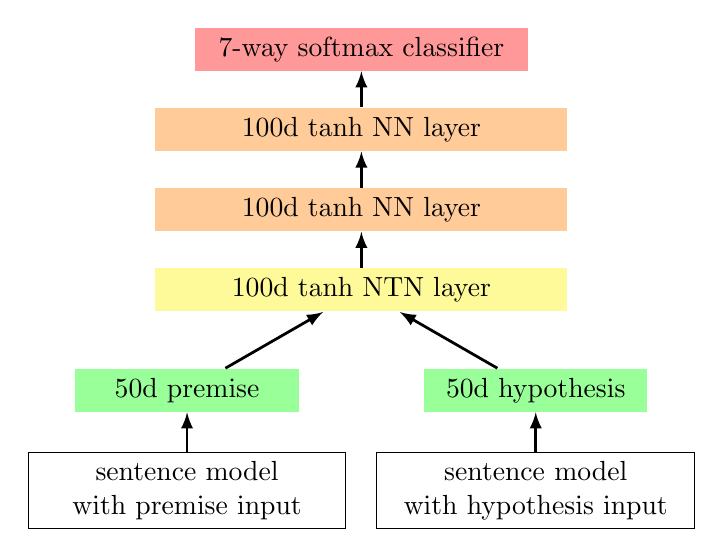
\begin{tikzpicture}
    \def\dx{21pt}
    \def\dy{29pt}

    \tikzstyle{label}=[text width=40mm,align=center]    
    \tikzstyle{softmax}=[fill=red!40,text width=40mm,align=center]
    \tikzstyle{preclass}=[fill=orange!40,text width=50mm,align=center]
    \tikzstyle{e}=[fill=green!40,text width=26mm,align=center]
    \tikzstyle{m}=[draw=black,text width=38mm,align=center]    
    
    \node[softmax]  (softmax) at (0*\dx,6*\dy) {7-way softmax classifier};
    \node[preclass]  (pc3) at (0*\dx,5*\dy) {100d $\tanh$ NN layer};
    \node[preclass]  (pc2) at (0*\dx,4*\dy) {100d $\tanh$ NN layer};
    \node[preclass,fill=yellow!40]  (pc1) at (0*\dx,3*\dy) {100d $\tanh$ NTN layer};
    \node[e]  (pe) at (-3*\dx,1.75*\dy) {50d premise};
    \node[e]  (he) at (3*\dx,1.75*\dy) {50d hypothesis};
    \node[m]  (pem) at (-3*\dx,0.5*\dy) {sentence model\\ with premise input};
    \node[m]  (hem) at (3*\dx,0.5*\dy) {sentence model\\ with hypothesis input};    
    
    \pgfsetarrowsend{latex}
    \tikzstyle{fwd} = [draw=black, line width=1pt]

          \draw [fwd] (pc3) -- (softmax);
          \draw [fwd] (pc2) -- (pc3);
          \draw [fwd] (pc1) -- (pc2);
          \draw [fwd] (pe) -- (pc1);
          \draw [fwd] (he) -- (pc1);
          \draw [fwd] (hem) -- (he);
          \draw [fwd] (pem) -- (pe);

  \end{tikzpicture}}
  
 \caption{The general architecture shared across models.}\label{fig:model:top}
  
\end{subfigure}

\begin{subfigure}[t]{0.45\textwidth}
  \centering
\scalebox{0.75}{
 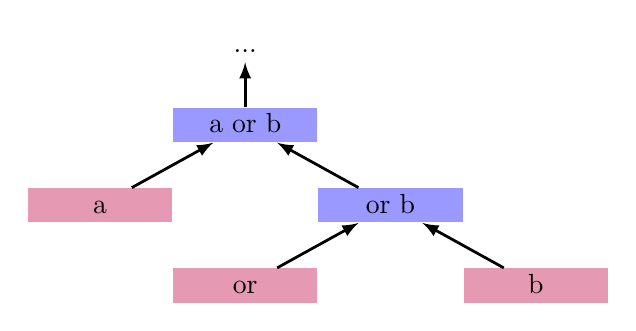
\begin{tikzpicture}
    \def\dx{21pt}
    \def\dy{29pt}


    \tikzstyle{word}=[fill=purple!40,text width=16mm,text height=2mm,align=center]
    \tikzstyle{node}=[fill=blue!40,text width=16mm,text height=2mm,align=center]
    \tikzstyle{empty}=[fill=blue!0,text width=8mm,text height=2mm,align=center]

    \node[empty]  (null) at (0*\dx,7*\dy) {...};
    \node[node]  (aorb) at (0*\dx,6*\dy) {a or b};
    \node[word]  (a) at (-2.5*\dx,5*\dy) {a};
    \node[node]  (orb) at (2.5*\dx,5*\dy) {or b};
    \node[word]  (or) at (0*\dx,4*\dy) {or};
    \node[word]  (b) at (5*\dx,4*\dy) {b};
    
    
    \pgfsetarrowsend{latex}
    \tikzstyle{fwd} = [draw=black, line width=1pt]

          \draw [fwd] (or) -- (orb);
          \draw [fwd] (b) -- (orb);
          \draw [fwd] (a) -- (aorb);
          \draw [fwd] (orb) -- (aorb);
          \draw [fwd] (aorb) -- (null);
  \end{tikzpicture}}
  
     \caption{The architecture for the TreeRNN and TreeRNTN sentence models. Terminal nodes are learned embeddings and nonterminal nodes are either NN or NTN layers with $\tanh$ nonlinearities.}\label{fig:model:tree}
  
  \end{subfigure}
 \vspace{0.5cm}
  
\begin{subfigure}[t]{0.45\textwidth}
  \centering
\scalebox{0.75}{
 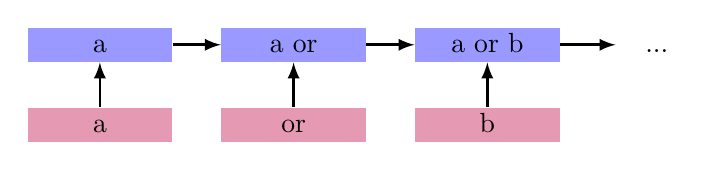
\begin{tikzpicture}
    \def\dx{35pt}
    \def\dy{29pt}


    \tikzstyle{word}=[fill=purple!40,text width=16mm,text height=2mm,align=center]
    \tikzstyle{node}=[fill=blue!40,text width=16mm,text height=2mm,align=center]
    \tikzstyle{empty}=[fill=blue!0,text width=8mm,text height=2mm,align=center]

    \node[word]  (a) at (-3*\dx,1*\dy) {a};
    \node[node]  (aN) at (-3*\dx,2*\dy) {a};
    
    \node[word]  (or) at (-1*\dx,1*\dy) {or};
    \node[node]  (orN) at (-1*\dx,2*\dy) {a or};
    
    \node[word]  (b) at (1*\dx,1*\dy) {b};
    \node[node]  (bN) at (1*\dx,2*\dy) {a or b}; 
    
    \node[empty]  (nullN) at (2.75*\dx,2*\dy) {...}; 
    
    \pgfsetarrowsend{latex}
    \tikzstyle{fwd} = [draw=black, line width=1pt]

          \draw [fwd] (or) -- (orN);
          \draw [fwd] (b) -- (bN);
          \draw [fwd] (a) -- (aN);
          \draw [fwd] (aN) -- (orN);
          \draw [fwd] (orN) -- (bN);
          \draw [fwd] (bN) -- (nullN);
          
  \end{tikzpicture}}
  
   \caption{The architecture for the LSTM sentence model. Nodes in the lower row are learned embeddings and nodes on the upper row are LSTM units.}\label{fig:model:seq}
  
    \end{subfigure}
  \caption{In our model, two copies of a sentence model---based on either tree (b) or sequence (c) models---encode the two sentences. A multilayer classifier component (a) then uses the resulting vectors to predict a label that reflects the logical relationship between the two sentences.}
  \label{sample-figure}
\end{figure}

\begin{figure*}[t]
  \centering
  \begin{subfigure}[t]{0.04\textwidth}
      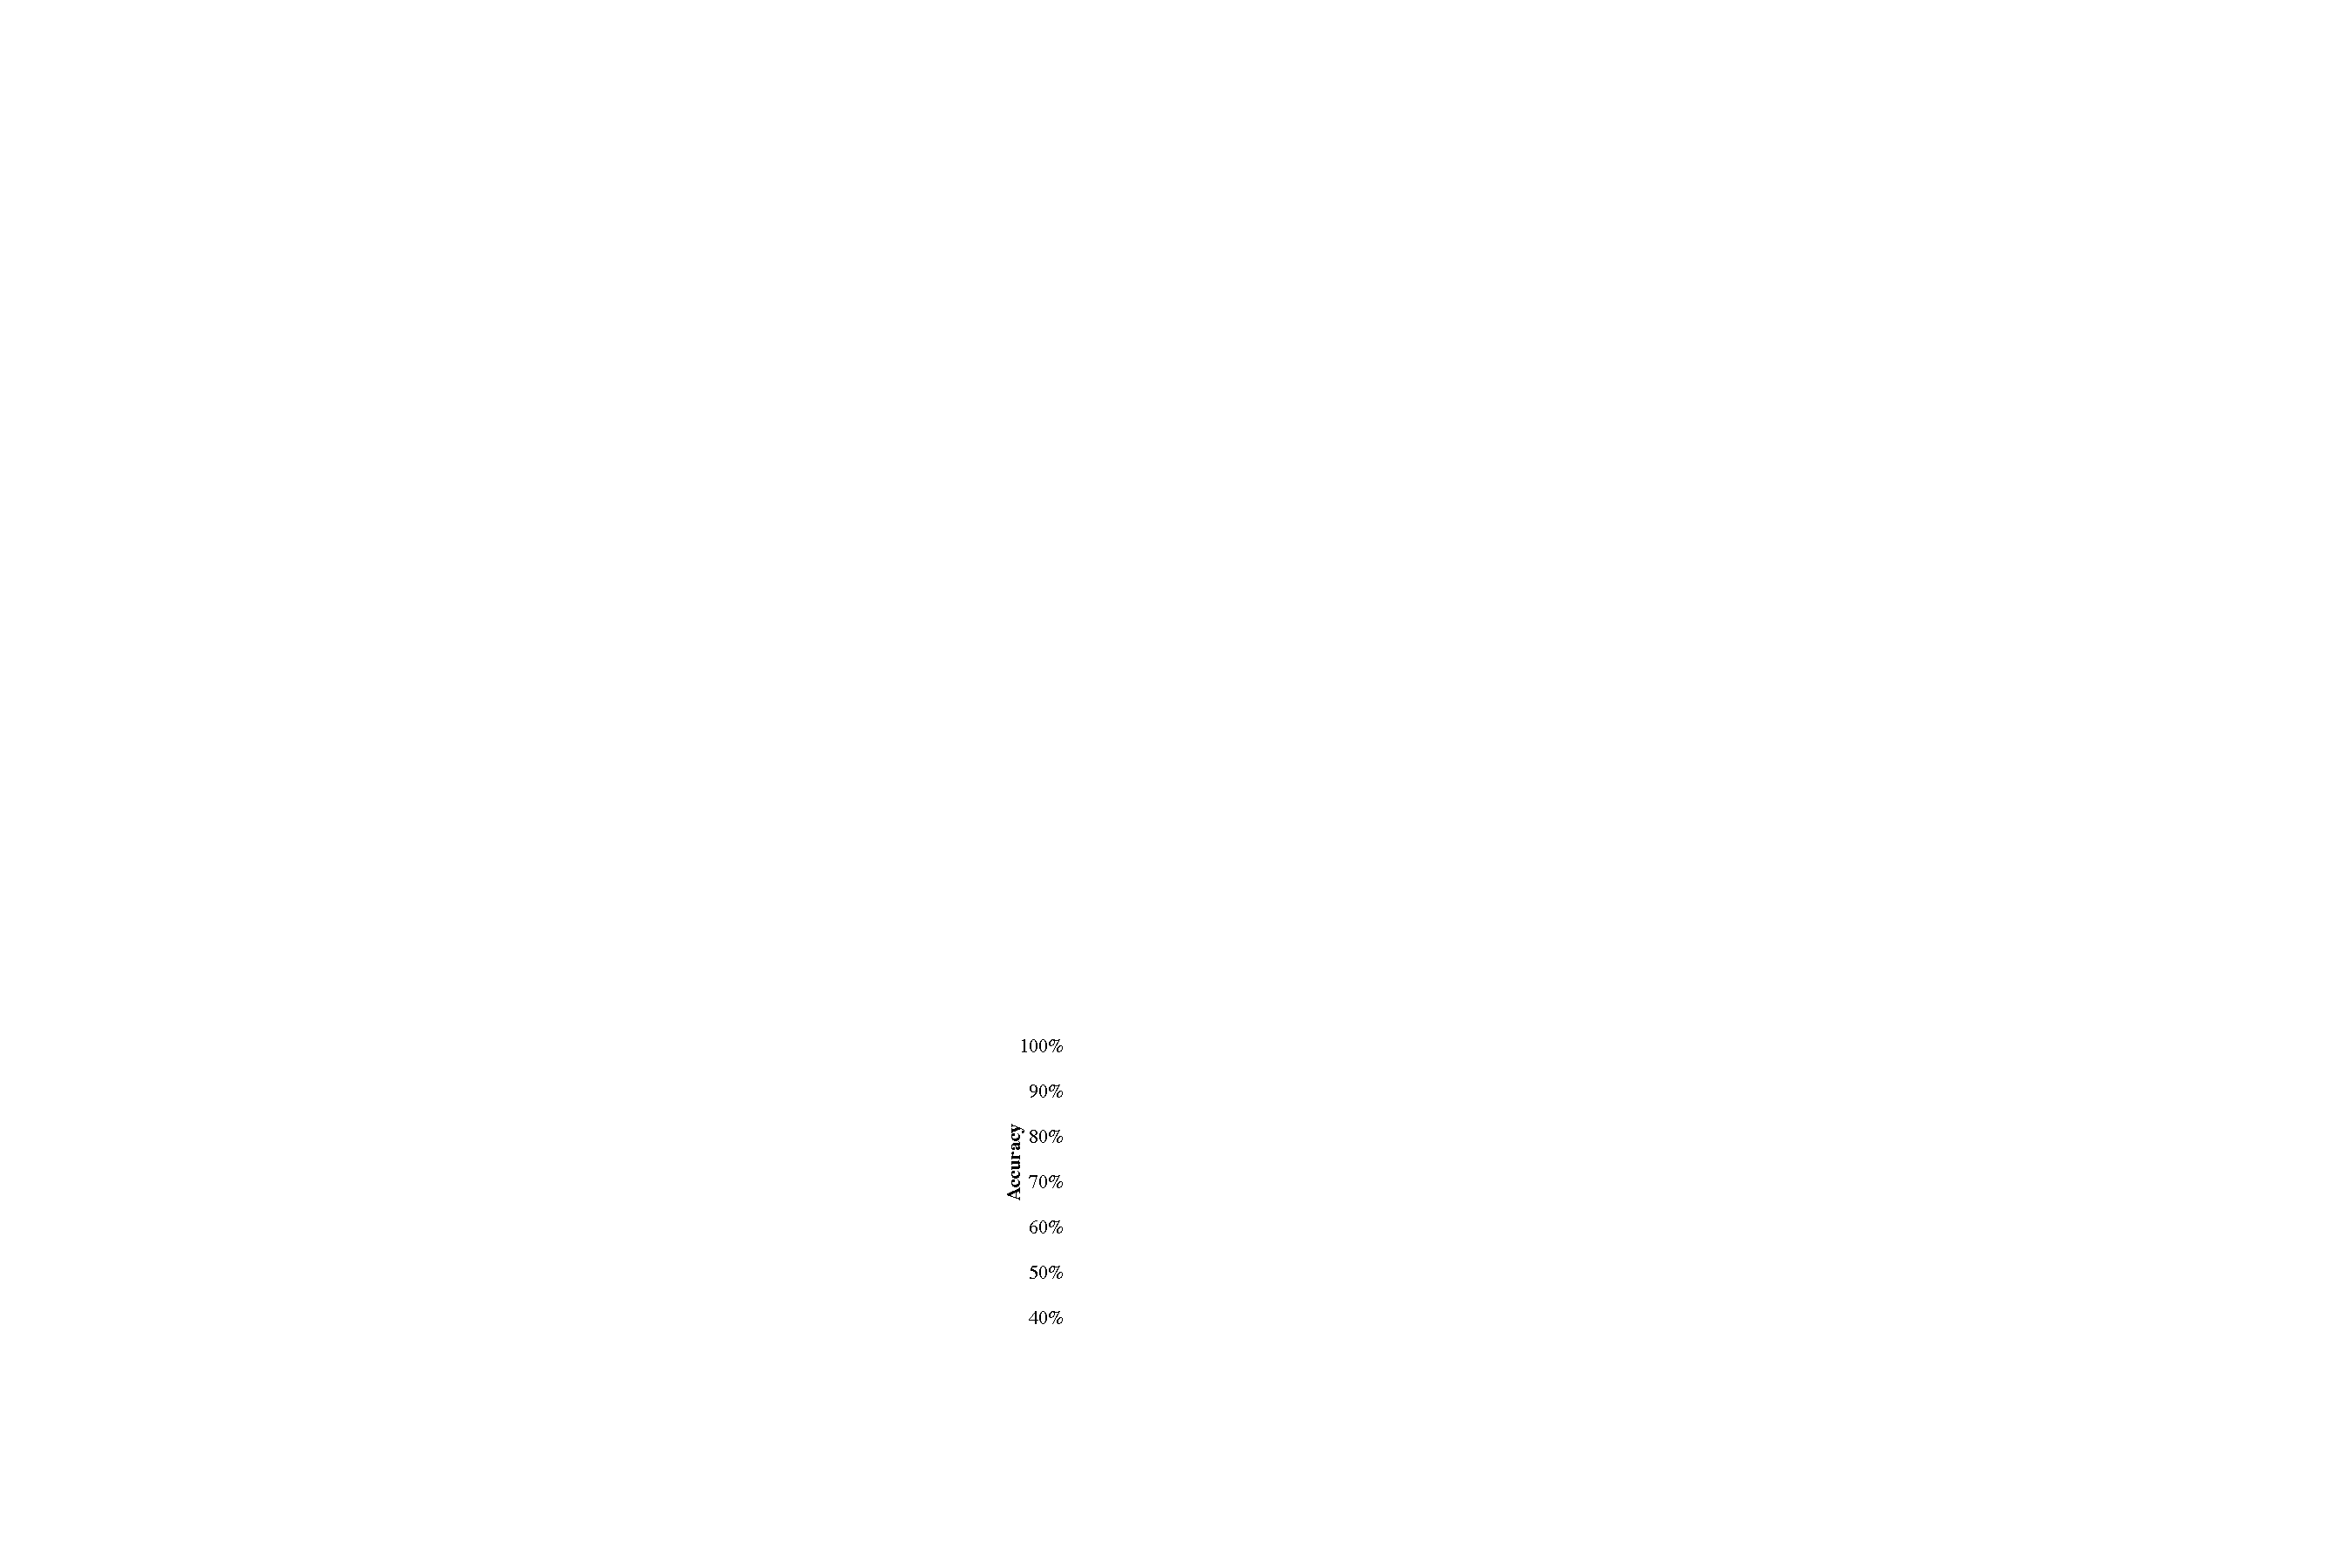
\includegraphics[height=1.5in]{scale.pdf}
\end{subfigure}
\begin{subfigure}[t]{0.24\textwidth}
  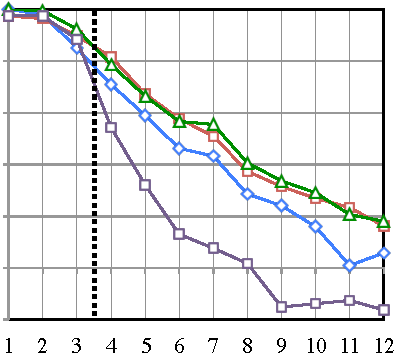
\includegraphics[height=1.5in]{fig3c.pdf}
  \caption{Training on sz. $\le$3.}
  \end{subfigure}~~~~
\begin{subfigure}[t]{0.24\textwidth}
    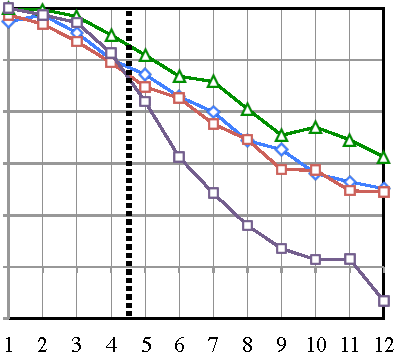
\includegraphics[height=1.5in]{fig4c.pdf}
  \caption{Training on sz. $\le$4.}
  \end{subfigure}~~~~
\begin{subfigure}[t]{0.24\textwidth}
      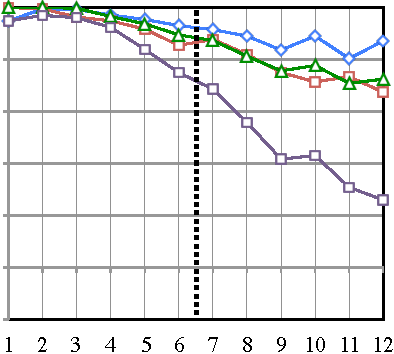
\includegraphics[height=1.5in]{fig6c.pdf}
  \caption{Training on sz. $\le$6.}
\end{subfigure}~~
\begin{subfigure}[t]{0.08\textwidth}
      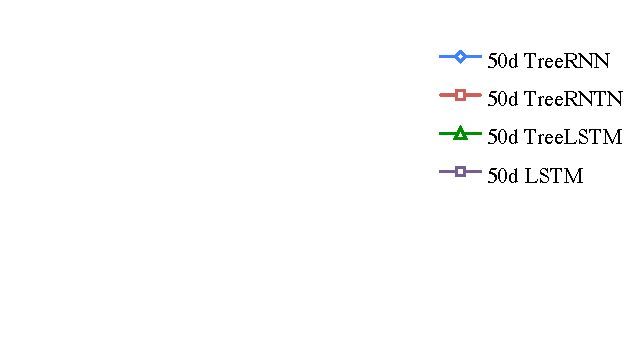
\includegraphics[height=1.5in]{leg.pdf}
\end{subfigure}
  \caption{Test accuracy on three experiments with increasingly rich training sets. The horizontal axis on each graph divides the test set expression pairs into bins by the number of logical operators in the more complex of the two expressions in the pair. The dotted line shows the size we trained on up to.}
  \label{prop-results} 
\end{figure*}

We use the architecture depicted in Figure~\ref{fig:model:top}, which builds on the one used in \newcite{Bowman:Potts:Manning:2014}. The model architecture uses two copies of a single sentence model (a tree or sequence model) to encode the premise and hypothesis (left and right side) sentences, and then uses those encodings as the features for a multilayer classifier which predicts one of the seven relations. Since the encodings are computed separately, the sentence models are forced to encode every element of the sentence meaning that the downstream model will need.

\paragraph{Classifier}
The classifier component of the model consists of a combining layer which takes the two sentence representations as inputs, followed by two neural network layers, then a softmax classifier.
For the combining layer, we use a neural tensor network (NTN, \citealt{chen2013learning}) layer, which sums the output of a plain recursive/recurrent neural network layer with a vector computed using two multiplications with a learned (full rank) third-order tensor parameter:
\begin{gather} 
\label{TreeRNN}
\vec{y}_{\textit{NN}} = \tanh(\mathbf{M} \colvec{2}{\vec{x}^{(l)}}{\vec{x}^{(r)}} + \vec{b}\,) \\
\label{TreeRNTN} 
\vec{y}_{\textit{NTN}} = \vec{y}_{\textit{NN}} + \tanh(\vec{x}^{(l)T} \mathbf{T}^{[1 \ldots n]} \vec{x}^{(r)})
\end{gather} 

Our model is largely identical to the Bowman et al.~model, but adds the two additional $\tanh$ NN layers, which we found help performance across the board, and also uses the NTN combination layer when evaluating all three models, rather than just the TreeRNTN model, so as to ensure that the three sentence models are compared in as similar a setting as possible.

\paragraph{Sentence models}
The sentence encoding component of the model transforms the (jointly learned) embeddings of the input words into a single sentence vector. We experiment with tree models (Figure~\ref{fig:model:tree}) with TreeRNN (eqn.~\ref{TreeRNN}), TreeRNTN (eqn.~\ref{TreeRNTN}), and TreeLSTM \cite{tai2015improved} activation functions. In addition, we use a sequence model (Figure~\ref{fig:model:seq}) with an LSTM activation function \cite{hochreiter1997long} implemented as in \newcite{zaremba2015recurrent}. Experiments with simpler non-LSTM RNN sequence models tended to underfit the training data, and are not included here.

\paragraph{Training} We randomly initialize all embeddings and layer parameters, and train them using minibatch stochastic gradient descent with AdaDelta \cite{zeiler2012adadelta} learning rates. Our objective is the standard negative log likelihood classification objective with L2 regularization (tuned on a separate train/test split). All models were trained for 72 epochs, after which all had largely converged without significantly declining from their peak performances.
